\documentclass[12pt]{article}
\usepackage[table,xcdraw]{xcolor}
\usepackage{graphicx,tabularx,ragged2e,float,pgfgantt,lscape,vhistory,listings,textcomp,fancyhdr,lastpage}
\usepackage[a4paper,left=3cm,right=3cm]{geometry}

\pagestyle{fancy}
\setlength{\headheight}{14.5pt}
\fancypagestyle{headerfooter} {
	\fancyhf{}
	\lhead{\footnotesize{Project Plan}}
	\rhead{\footnotesize{Version 3.0}}
	\lfoot{\footnotesize{Aberystwyth University / Computer Science}}
	\rfoot{\footnotesize{Page \thepage~of \pageref{LastPage}}}
}

\definecolor{lgreen}{HTML}{AEE59B}
\definecolor{dgreen}{HTML}{6DAE56}
\definecolor{sgreen}{HTML}{F5F5F5}

\definecolor{dkgreen}{rgb}{0, .6, 0}
\definecolor{dkblue}{rgb}{0, 0, .6}

\definecolor{dkyellow}{cmyk}{0, 0, .8, .3}

\lstset{
    language			= php,
		basicstyle		= \small\ttfamily,
    keywordstyle	= \color{dkblue},
    stringstyle		= \color{red},
    identifierstyle	= \color{dkgreen},
    commentstyle	= \color{gray},
    emph				=[1]{php},
    emphstyle		=[1]\color{black},
    emph				=[2]{if,and,or,else},
    emphstyle		=[2]\color{dkyellow}}

\newcolumntype{Y}{>{\RaggedRight\arraybackslash}X}

\title{Group 9 \protect\\ Project Plan}
\author{Anna Laura Zielinska \and John Batty \and John Friend \and Jack Cridland \and Kamil Lewinsky \and Leon Hassan \and Punit Shah \and Rowan Alexander}
\date{9\textsuperscript{th} February 2015}

\begin{document}

\maketitle
\thispagestyle{headerfooter}
\pagestyle{headerfooter}

\begin{center}
	Config Ref: SE\_09\_PP\_01\\
	Version: 3.0\\
	Status: Release\\
	~\\
	Department of Computer Science\\
	Aberystwyth University\\
	Aberystwyth\\
	Ceredigion\\
	SY23 3DB\\
	Copyright \textcopyright~Aberystwyth University
\end{center}

\clearpage

\tableofcontents
\clearpage

\section{Introduction}

	\subsection{Purpose of this Document}
		The purpose of this document is to describe how we will accomplish the project, by deriving a set of objectives from the requirements specification.
	\subsection{Scope}
		This document details the project's resources, proposed system and schedule.\\
		This document is intended to be read by the client to ensure we have correctly understood the requirements.
	\subsection{Objectives}
		\begin{enumerate}
			\item To provide a description of the system components, how they interact with each other, our choice of platforms, and the target users
			\item To describe how the clients will interact with the system
			\item To illustrate the appearance of the user interfaces and the effects of interaction with interface elements
			\item To describe major tasks, as well as which group member is responsible for each task and the schedule for the task's completion
			\item To identify the main issues we may encounter and how we would respond to them
		\end{enumerate}

\section{Overview of proposed system}

	\subsection{System components and platforms}
		The system will be comprised of the following components:
		\begin{itemize}
			\item An Android app (RPSRrec) for making species recordings in the field. The device will transmit the recordings to the server (RPSRsrv) as soon as a network connection is provided. We will use Android Studio to develop the app.
			\item A server (RPSRsrv) that will receive transmissions from the RPSRrec Android app and then add them to database. This will be implemented as a PHP script that will receive HTTP POST requests sent from the app and adding the relevant data to the database with SQL commands. The database management system we will use is MySQL.
			\item A website (RPSRview) which allows the user to browse species records, as well as add and maintain reserves. This will be implemented using PHP.
		\end{itemize}

	\subsection{Target user characteristics}
		The system will be used by naturalists who are familiar with standard computer interfaces, and may use this system in difficult weather conditions and remote locations.\\
		A user may be simply a regular user that will use the RPSRrec Android app to make recordings in the field, and the RPSRview website to browse species records.\\
		A user may also be an administrator that has permission to add and maintain reserve data using the RPSRview website.

\section{Use-cases}
	Figure~\ref{fig:use-case-diagram} on page~\pageref{fig:use-case-diagram} shows the use case diagram for the system's clients and describes the use cases of clients including both users and the Android device. They are separated into the subsystems that the clients can interact with: the RPSRrec Android app, the RPSRview website and the Android operating system.

	\begin{figure}[H]
		\begin{center}
			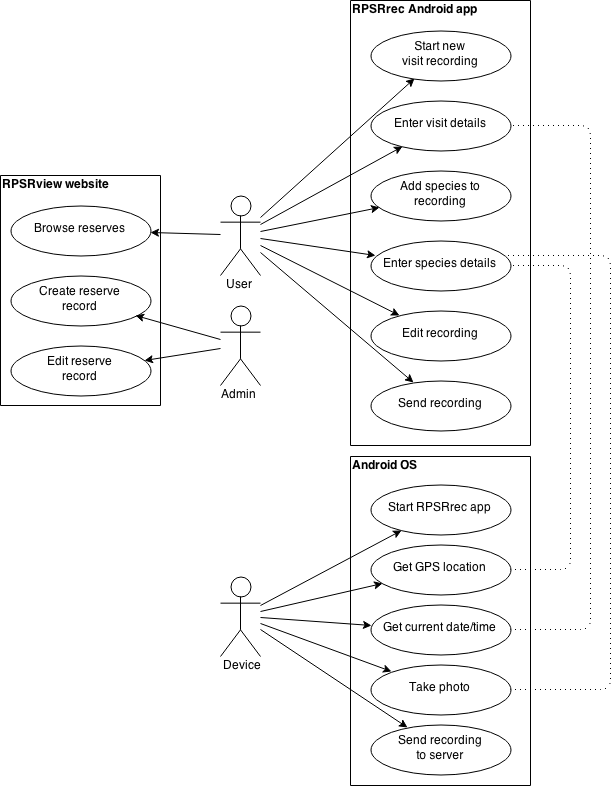
\includegraphics[scale=0.5]{use-cases}
		\end{center}
		\caption{Client use-cases}
		\label{fig:use-case-diagram}
	\end{figure}

	\subsection{RPSRrec Android app}
		\subsubsection{Start new visit recording}
			Upon starting the app, the user will be able to start a new visit recording. The user will then be asked to enter details of their visit (see section~\ref{sec:enter-visit-details}).
		\subsubsection{Enter visit details}
			\label{sec:enter-visit-details}
			The user will select the name of the reserve they are visiting from a list, followed by their own name, phone number and e-mail address. The user will not need to enter information about the date and time as these details will be obtained from the Android device (see section~\ref{sec:get-date-time}).
		\subsubsection{Add species to recording}
			The user will be able to search for a species from a list and select it to be added to the recording. If the species is not in the list, they will be given the option to provide a new species.\\
			The user may select more than one species.
		\subsubsection{Enter species details}
			\label{sec:enter-species-details}
			Once a species has been added to the recording, the user will be prompted to add details about the species.\\
			These details include the following.
			\begin{itemize}
				\item A location for the species within the site\\
				The user will not ordinarily need to provide any input for this as the location will be recorded using the device's GPS receiver (see section~\ref{sec:get-gps}). However, in the event of GPS being disabled on the device, the user will be prompted to turn it on.
				\item The abundance of the species\\
				The user will be able to enter an abundance using the "DAFOR" scale.
				\item A free text comment\\
				The user will be able to enter a comment to describe the species. The inclusion of this detail is optional.
				\item A photo of the general scene at the location of the species\\
				The user will be able to either take a photo of the location using the device's camera (see section~\ref{sec:take-photo}), or choose an existing photo from the device's photo gallery. The inclusion of this photo is optional.
				\item A photo of the specimen\\
				As above, except the user will be asked to provide a photo of the specimen. The inclusion of this photo is also optional.
			\end{itemize}
		\subsubsection{Edit recording}
			Once the user has finished adding species to the recording, they will be given the option to edit the recording. They will be able to edit it in the following ways:
			\begin{itemize}
				\item Deleting the whole recording
				\item Deleting one of the species in the recording
				\item Changing the details of one of the species in the recording
			\end{itemize}
		\subsubsection{Send recording}
			Once the user has finished editing the recording, they can send the recording to the server. The device will need to be connected to the internet in order to do this. If no connection is available, a message will be displayed and the user will be able to retry once they are connected.

	\subsection{RPSRview website}
		\subsubsection{Browse reserves}
			The web interface will allow the user to select a reserve and view a complete list of species recorded at that reserve. The list of species will be ordered alphabetically by their Latin name. The user will be given the option to order the list by date instead.\\
			As well as the name of the species, each item in the list will also contain the recorder's name, the date, and the abundance. Users will be given the option to view any associated photos of the species and the general scene.
		\subsubsection{Create reserve record}
			Once authenticated, the administrator will be able to create a new reserve record. For each new reserve record, they will be required to enter the following information:
			\begin{itemize}
				\item The reserve's name
				\item The location of its principle access point as an OS grid reference
				\item A textual description
			\end{itemize}
		\subsubsection{Edit reserve record}
			Once authenticated, the administrator will also be able to update the details of a reserve, or entirely delete its record.

  \subsection{Android OS}
  	\subsubsection{Start RPSRrec app}
  		The RPSRrec app will be launched from the Android device's apps.
    \subsubsection{Get GPS location}
    	\label{sec:get-gps}
    	The GPS receiver of the device will be used to determine the location of the species during a recording (see section~\ref{sec:enter-species-details}).
  	\subsubsection{Get current date/time}
  		\label{sec:get-date-time}
  		The operating system will get the current date and time from the device's calendar. This will be used when entering details of the visit (see section~\ref{sec:enter-visit-details}).
    \subsubsection{Take photo}
    	\label{sec:take-photo}
    	The device's camera will be used to take photographs of the specimen and of the general scene at the location of the specimen (see section~\ref{sec:enter-species-details}).
    \subsubsection{Send recording to server}
    	When connected to the internet, the device will send the recording data to the server.

\section{User interface design}
	\subsection{Website design}
		Design is key where websites are concerned, this is why you have to make sure that the user knows the outcomes to the interaction they have with the site, they know what the site is used for, where they are in the site and how do they move around the site. These key points can basically make or break a site so design in a website must be looked into with detail and with a complete open mind. The plans which have been created have met these points as they make sure that the user knows where they are and how to move around. But not only that, the design shouldn’t make the user “switch off” when they are using our site.
		
		The Bootstrap framework will be used to generate our CSS. The reason behind using Bootstrap is because it ensures clean and professional looking sites, and has a grid theme which helps the creator of the site build on top of. Almost like blueprints for where everything should go. But most importantly, it works very well with PHP. PHP is a great scripting language, but when it comes to generating HTML, it can get quite messy. With Bootstrap's grid system, this makes it hard for generated HTML tags and information to be in the wrong area.

		The way which the site is going to be generated is by having 4 files (minus the potential PHP classes for database connection). These 4 files are index, header, core and footer.

		The idea is to generate all of your pages on-the-fly, in one php file. This isn't ethical programming (from an object oriented standpoint), but this is in web development. The only code that our index page will require is: 

	  \begin{lstlisting}[language=php]
	  <?php
	    require_once ‘header.php’;
	    require_once ‘core.php’;
	    require_once ‘footer.php’;
	  ?>
	  \end{lstlisting}

	  This code loads up the three main components of the page and loads it into the current page, this means that the actual page you are on does not change at all on your visit. The page actually acts as a shell for which we then load information into for the user. The header and footer files will be the same for all pages but the core will not. The core will have all the functions, variables, methods etc, so that the site is being generated and understands where the user currently is in the site.

	  The way the user progresses through the site is dependent on their current location. What this means is if the user is looking at the list of reserves, they won’t be able to jump to a specimen without firstly going into the reserves array, selecting one, and then selecting the specimen they wish to see. The way this is possible is by using the \texttt{if(isset(\$\_GET['']))} method. Which will run if the string which the method is looking for appears in the URL bar. This will allow the creators of the site to call reference keys on records, which in return generate the pages we need. The main way the user will navigate through the site is by clicking on generate hyperlinks which will basically show more and more information the deeper you go. What this means is that the user will have the entire array of reserves on show. The user won’t be able to view what is inside that reserve until they click on the name of it. From there, all of the species will be shown to the user with basic information being: Specimen name, Common name and Date (It was recorded). The only way the user can see more information is by, again, clicking on the name of the specimen they want to see. Thus revealing all the possible data about that one specimen. Also to add, the name of the page the user will be on, will always be the same location (top left of the screen, under the NavBar) this will ensure the user will know where to look if they become lost in the site and to actually let the user know what part of the site they are on.

	  \begin{figure}[H]
			\begin{center}
				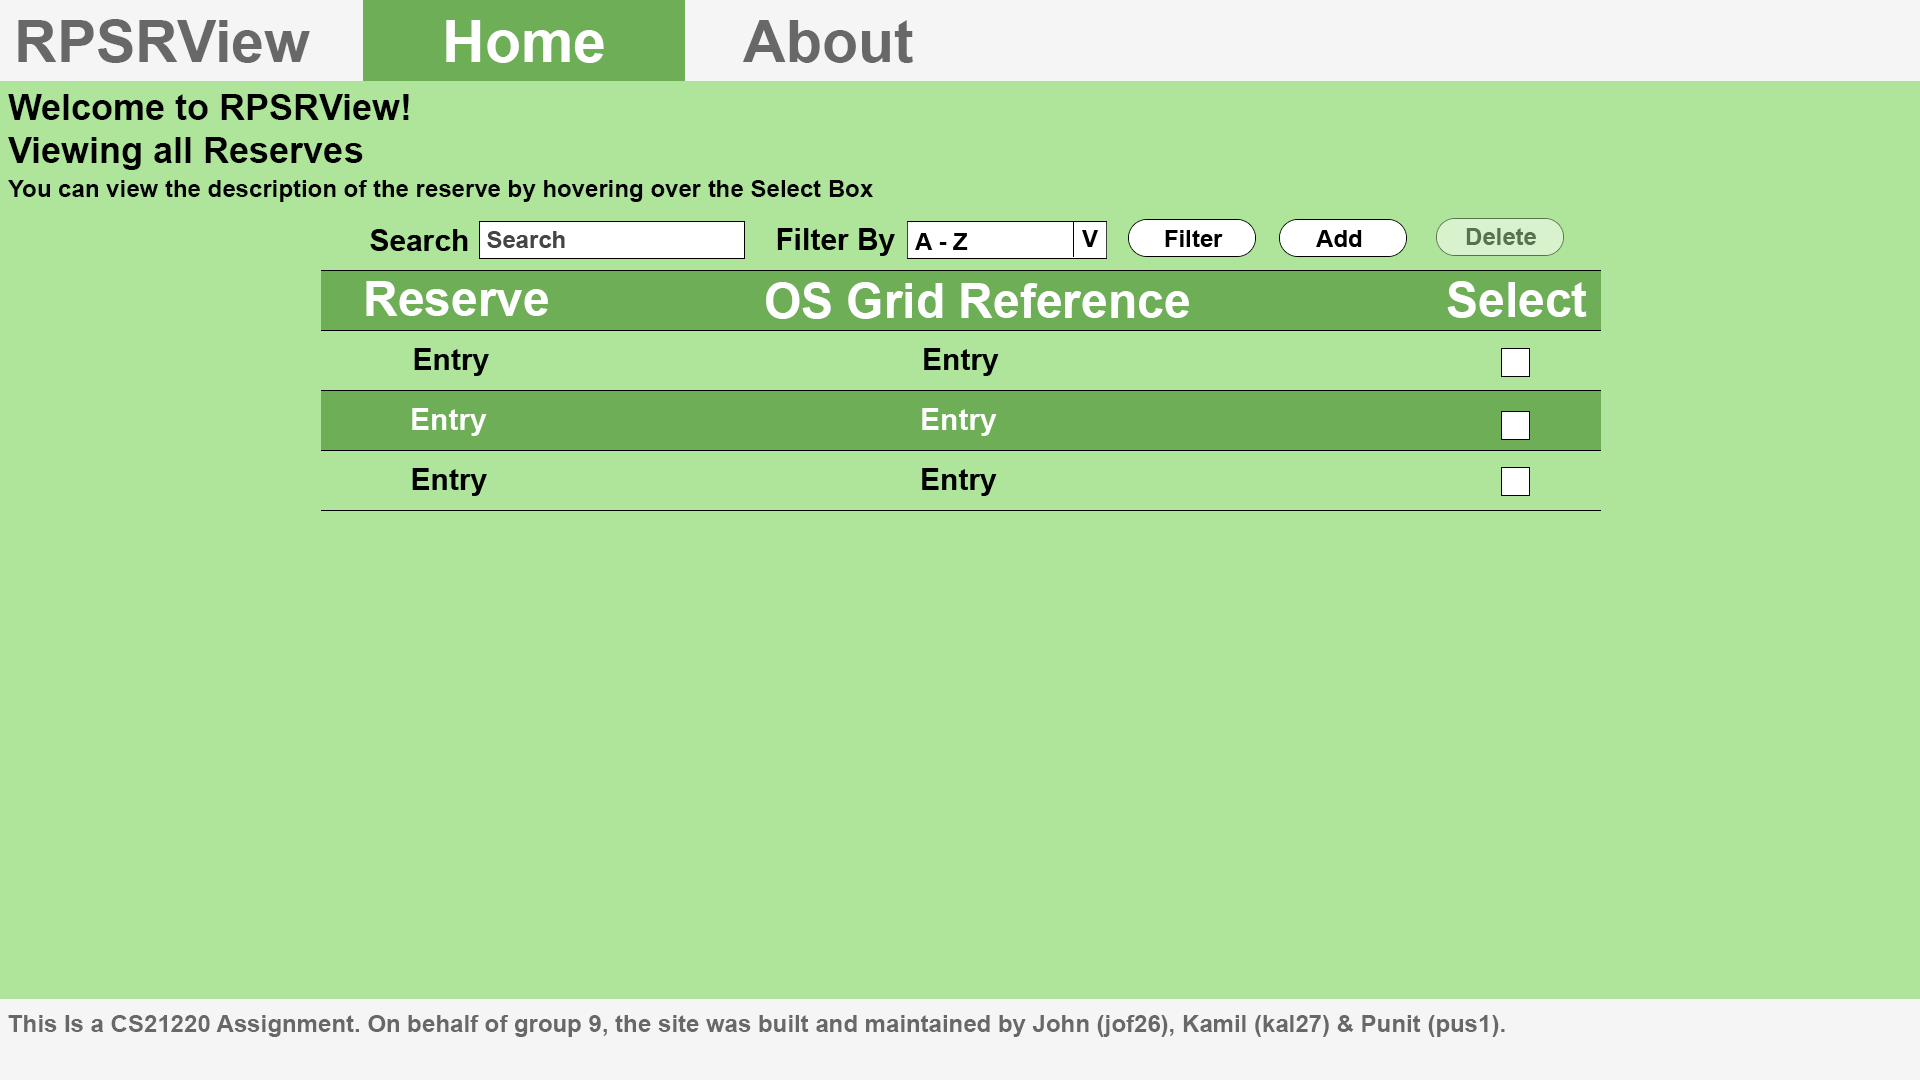
\includegraphics[scale=0.20]{web-IndexPLAN}
			\end{center}
			\caption{Index page}
			\label{fig:index-page}
		\end{figure}

	  \noindent The aim for the design of the site was to make sure it is clean looking and it doesn’t confuse the user, considering it is made to display confusing data so it would be a bad idea to further confuse them with a site which doesn’t behave naturally. The way this can be achieved is by making sure each page looks similar to the rest. Once the user knows where they are and what the site looks like, you don’t want to be throwing them off by completely changing the house style of the site.

	  There will be a navigation bar at the top of the page, fixed position, that will help the user switch back to the home page or to the about page, very quickly, which could be needed if the user doesn’t want to look at specimen in the current reserve but wants to look at one in another. It will also display the name of the site to them ensure them that they haven’t left the site when they click on a hyperlink to navigate the site.

		\begin{itemize}
			\item Light Green (\textcolor{lgreen}{\texttt{\#AEE59B}}) for the background
			\item Dark Green (\textcolor{dgreen}{\texttt{\#6DAE56}}) for borders and details
			\item White (\texttt{\#FFFFFF}) for the background of text (eg. main content of the Index page in Figure~\ref{fig:index-page})
	  	\item Black (\texttt{\#000000}) for the actual text
		\end{itemize}

		\noindent These colours were chosen because, being a site with botanists as the target audience, it seems natural to have a tint of green to symbolise plants. The scheme for these two colours are that the light green will be placed as a background primarily. Whereas the dark green will be used as a highlighter, for the tables and for the navigation bar. This will help the user distinguish where they are at any time. You will notice in Figure~\ref{fig:index-page} that the mouse is hovering over the second entry of the table, which is making the whole row highlight the dark green, and changing the font colour. This happens for the navigation bar also.

		\begin{figure}[H]
			\begin{center}
				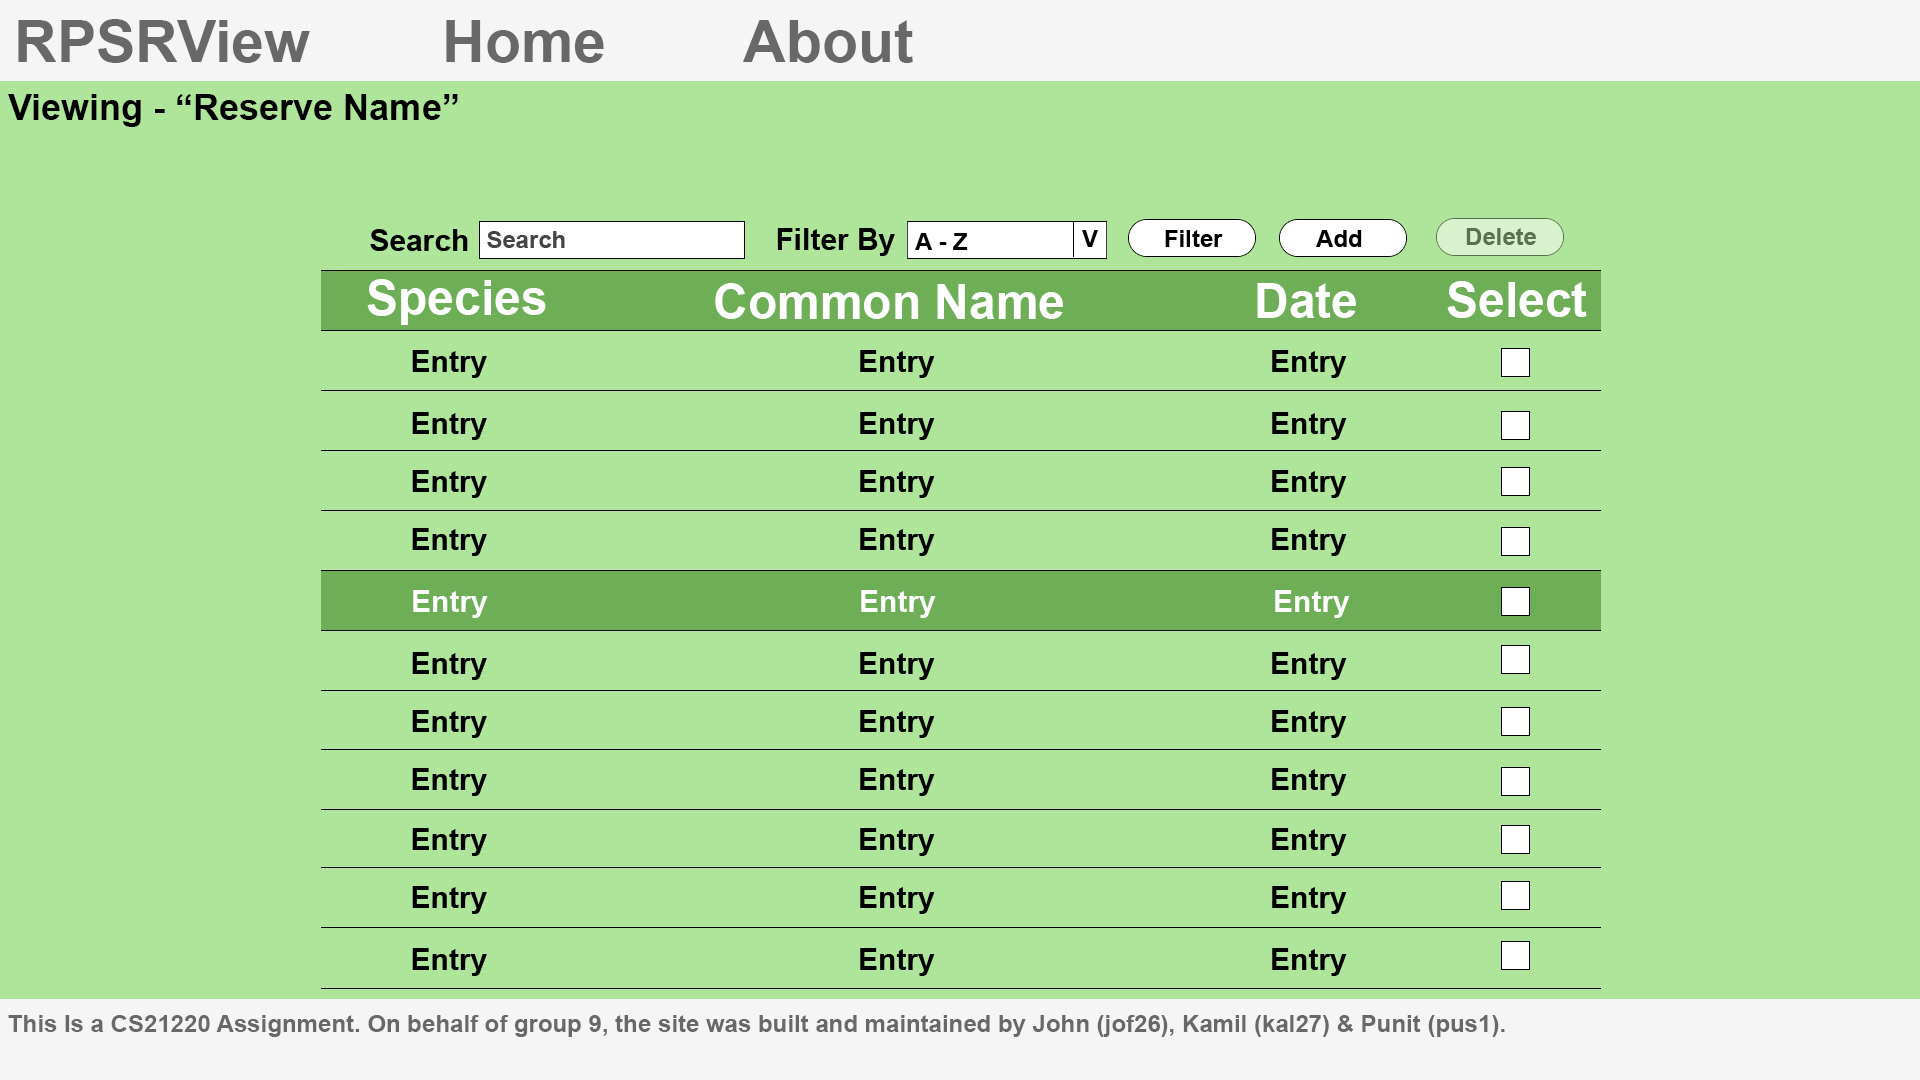
\includegraphics[scale=0.20]{web-InsideReservePLAN}
			\end{center}
			\caption{Inside Reserve page}
			\label{fig:ireserve-page}
		\end{figure}

		\noindent The footer and header have a background colour which isn’t either of the greens, nor is it white. It is in fact \texttt{\#F5F5F5}. Using this colour instead of complete white (\texttt{\#FFF}) will help highlight the areas we need the user to see, which will be in the centre of the screen. So when there is text which is white or black, they will stand out more, instead of the user being drawn to these two blinding white blocks at the top and bottom of the screen.

		\begin{figure}[H]
			\begin{center}
				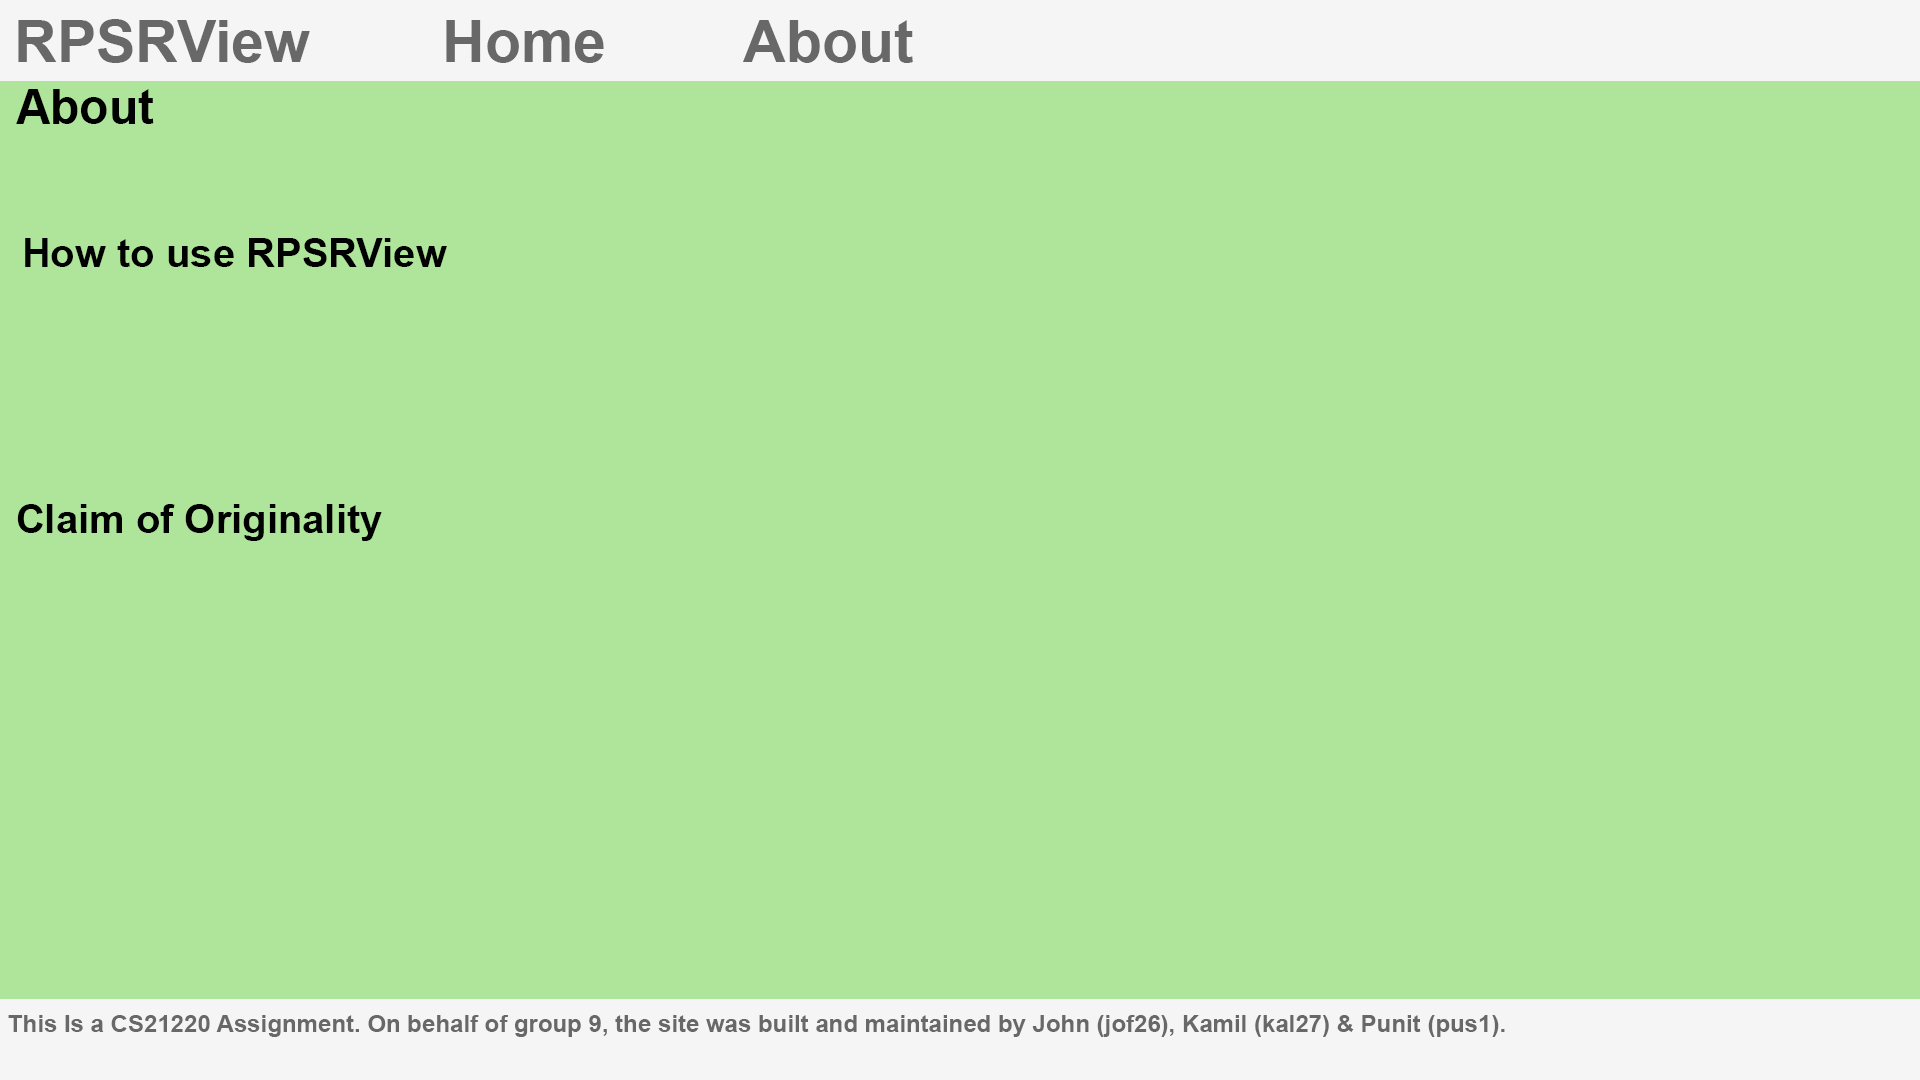
\includegraphics[scale=0.20]{web-AboutPLAN}
			\end{center}
			\caption{About page}
			\label{fig:about-page}
		\end{figure}

		\noindent When the user wants to add a specimen, they will have to navigate to the InsideReserve page. From there, the user will simply click the \textbf{Add} button located above the table. Here the user will be able to fill in the required data, which will be validated using HTML5's form checking to make sure the data is correct at a basic level. The Abundance field will be a drop-down box to further stop human error on the user's behalf by inputting wrong data into the system. Similarly, the user can edit the specimen. They do this by navigating to the specimen they wish to edit. And from there, click on the \textbf{Edit} button located at the top of the page. This link will take the user to a page which will look similar to the \textbf{Add} specimen page. However, the data in the HTML forms will already have data in them, this being the same data the user saw in the last page. But this time the user can click on the forms which they want to edit and click on the Save Changes button located at the top of the page again. This will throw out a pop up message (alert) to say the changes have been saved and updated.

		\begin{figure}[H]
			\begin{center}
				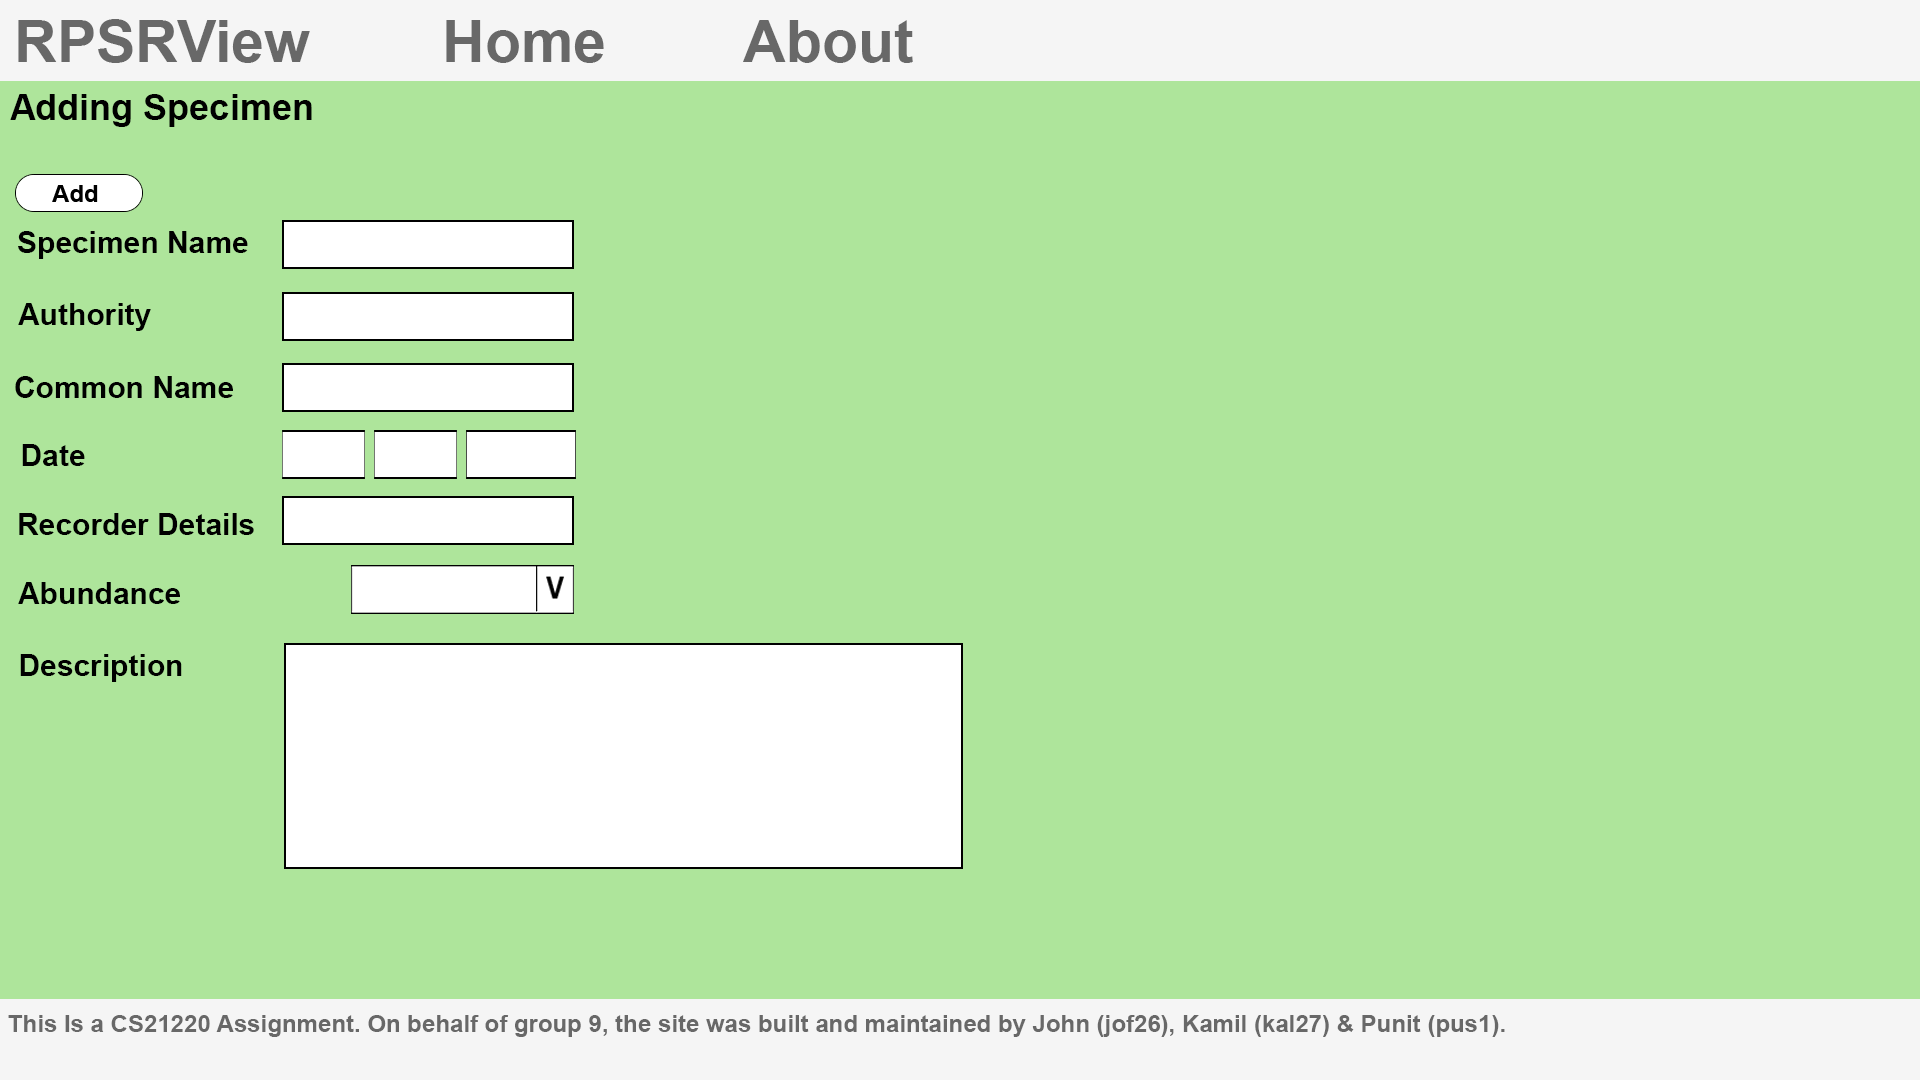
\includegraphics[scale=0.20]{web-AddSpecimenPLAN}
			\end{center}
			\caption{Add Specimen page}
			\label{fig:adds-page}
			\begin{center}
				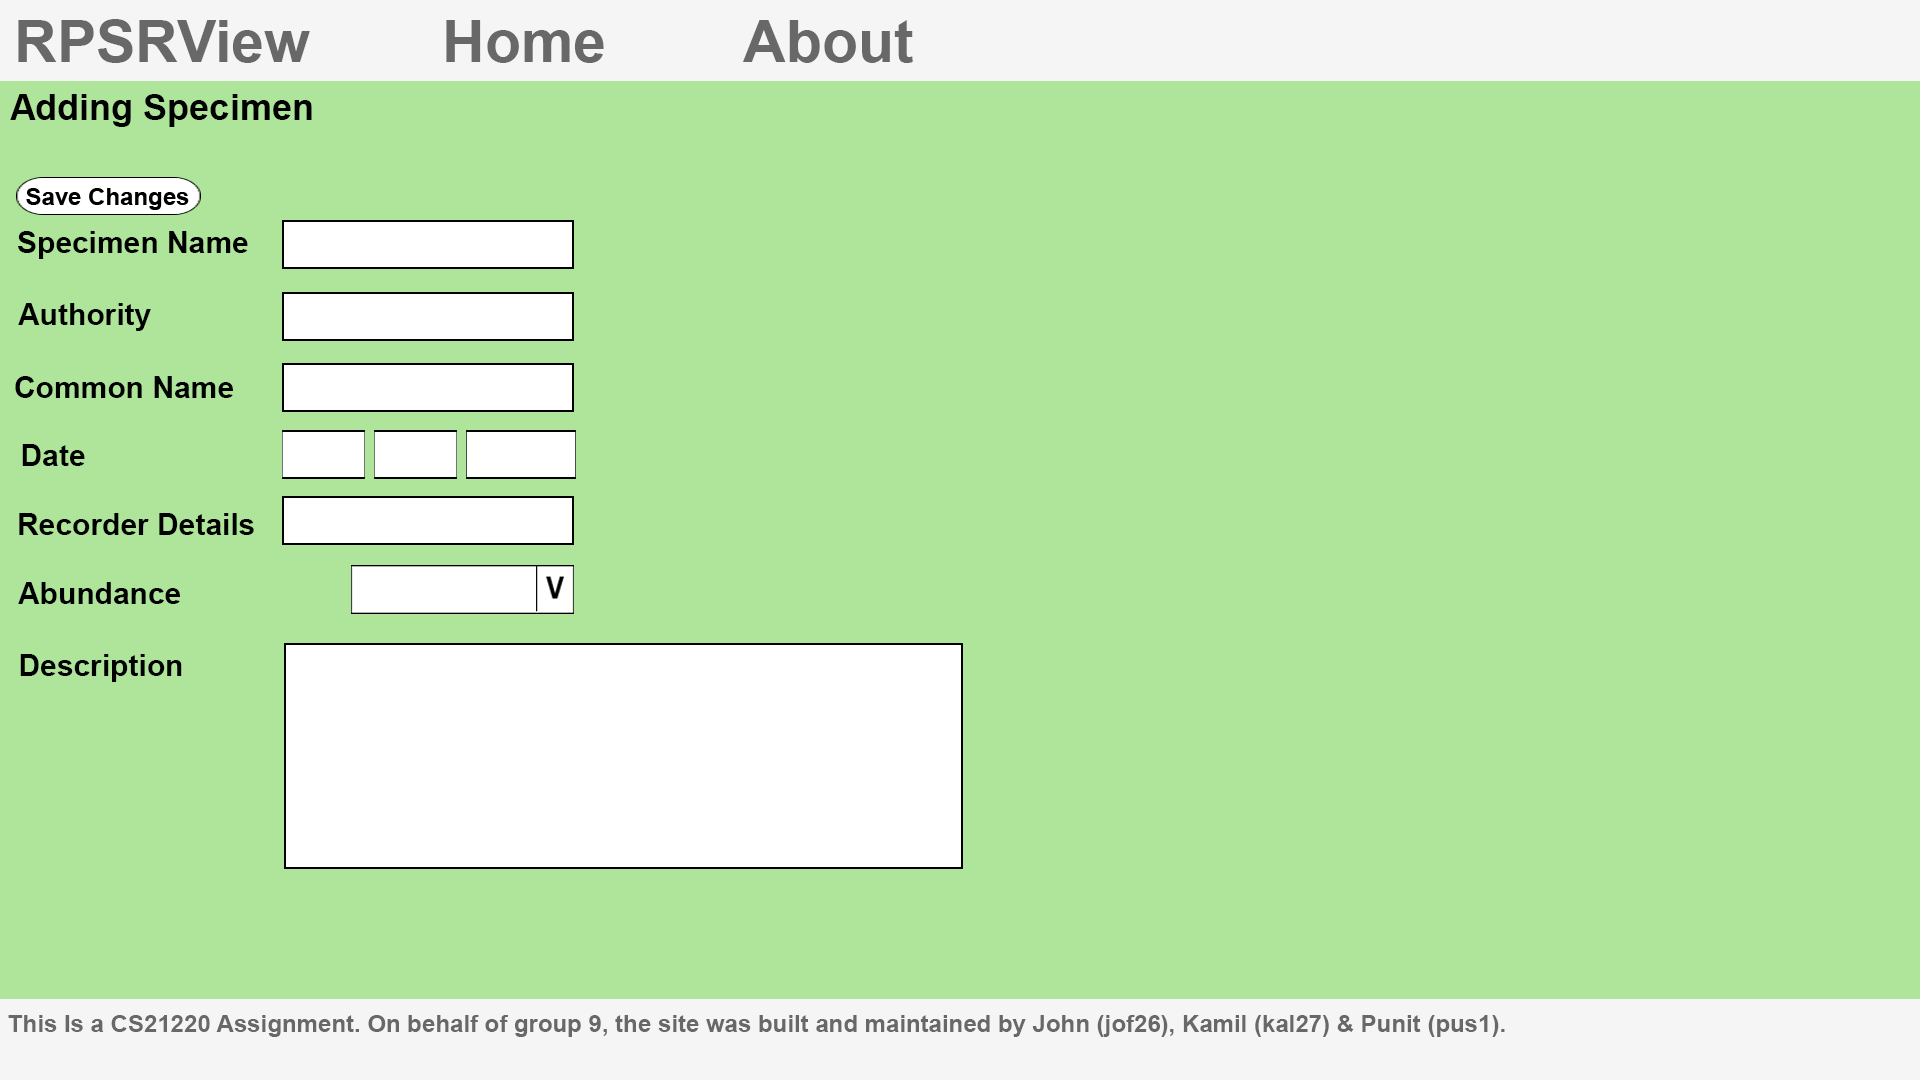
\includegraphics[scale=0.20]{web-EditSpecimenPLAN}
			\end{center}
			\caption{Edit Specimen page}
			\label{fig:edits-page}
		\end{figure}

		\noindent Do note that in the images shown in this section have some areas which have objects in them which have 50\% opacity. This is because they are dependent on other parts of the page. The \textbf{Delete} button (found in Index (Figure~\ref{fig:index-page}) and Inside Reserve (Figure~\ref{fig:ireserve-page})) will only show when the user clicks on the tick box on the row of the reserve or specimen they which to delete. There is another object which is found on this page, these images are also dependant because the number of photos you can attach to a specimen range from 0 to many (no hard limit as of yet). It could have 1, 4, 30, or it could have none.

		\begin{figure}[H]
			\begin{center}
				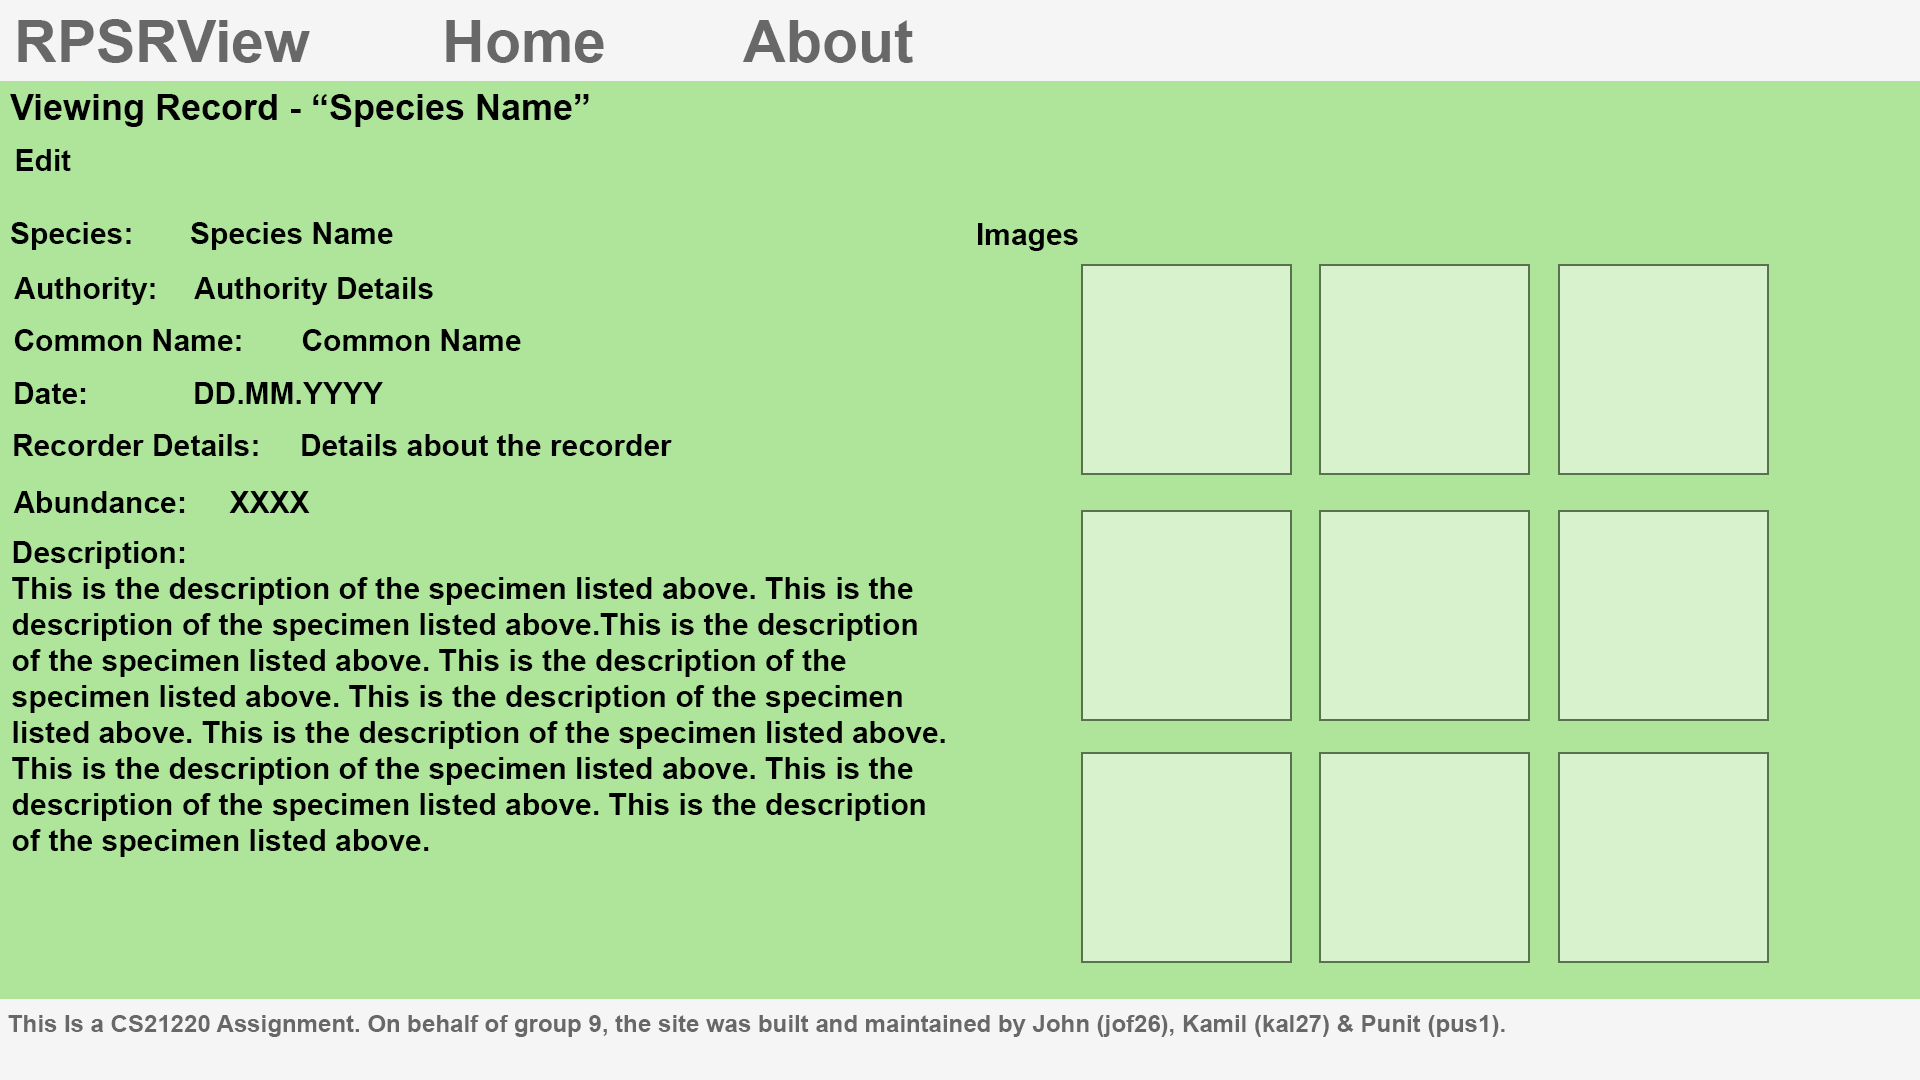
\includegraphics[scale=0.20]{web-InsideSpecimenPLAN}
			\end{center}
			\caption{Specimen Details page}
			\label{fig:details-page}
		\end{figure}

		\noindent The page flow diagram (Figure~\ref{fig:pflow-page}) shows how the pages are linked and how a user can navigate from page to page.

		\begin{figure}[H]
			\begin{center}
				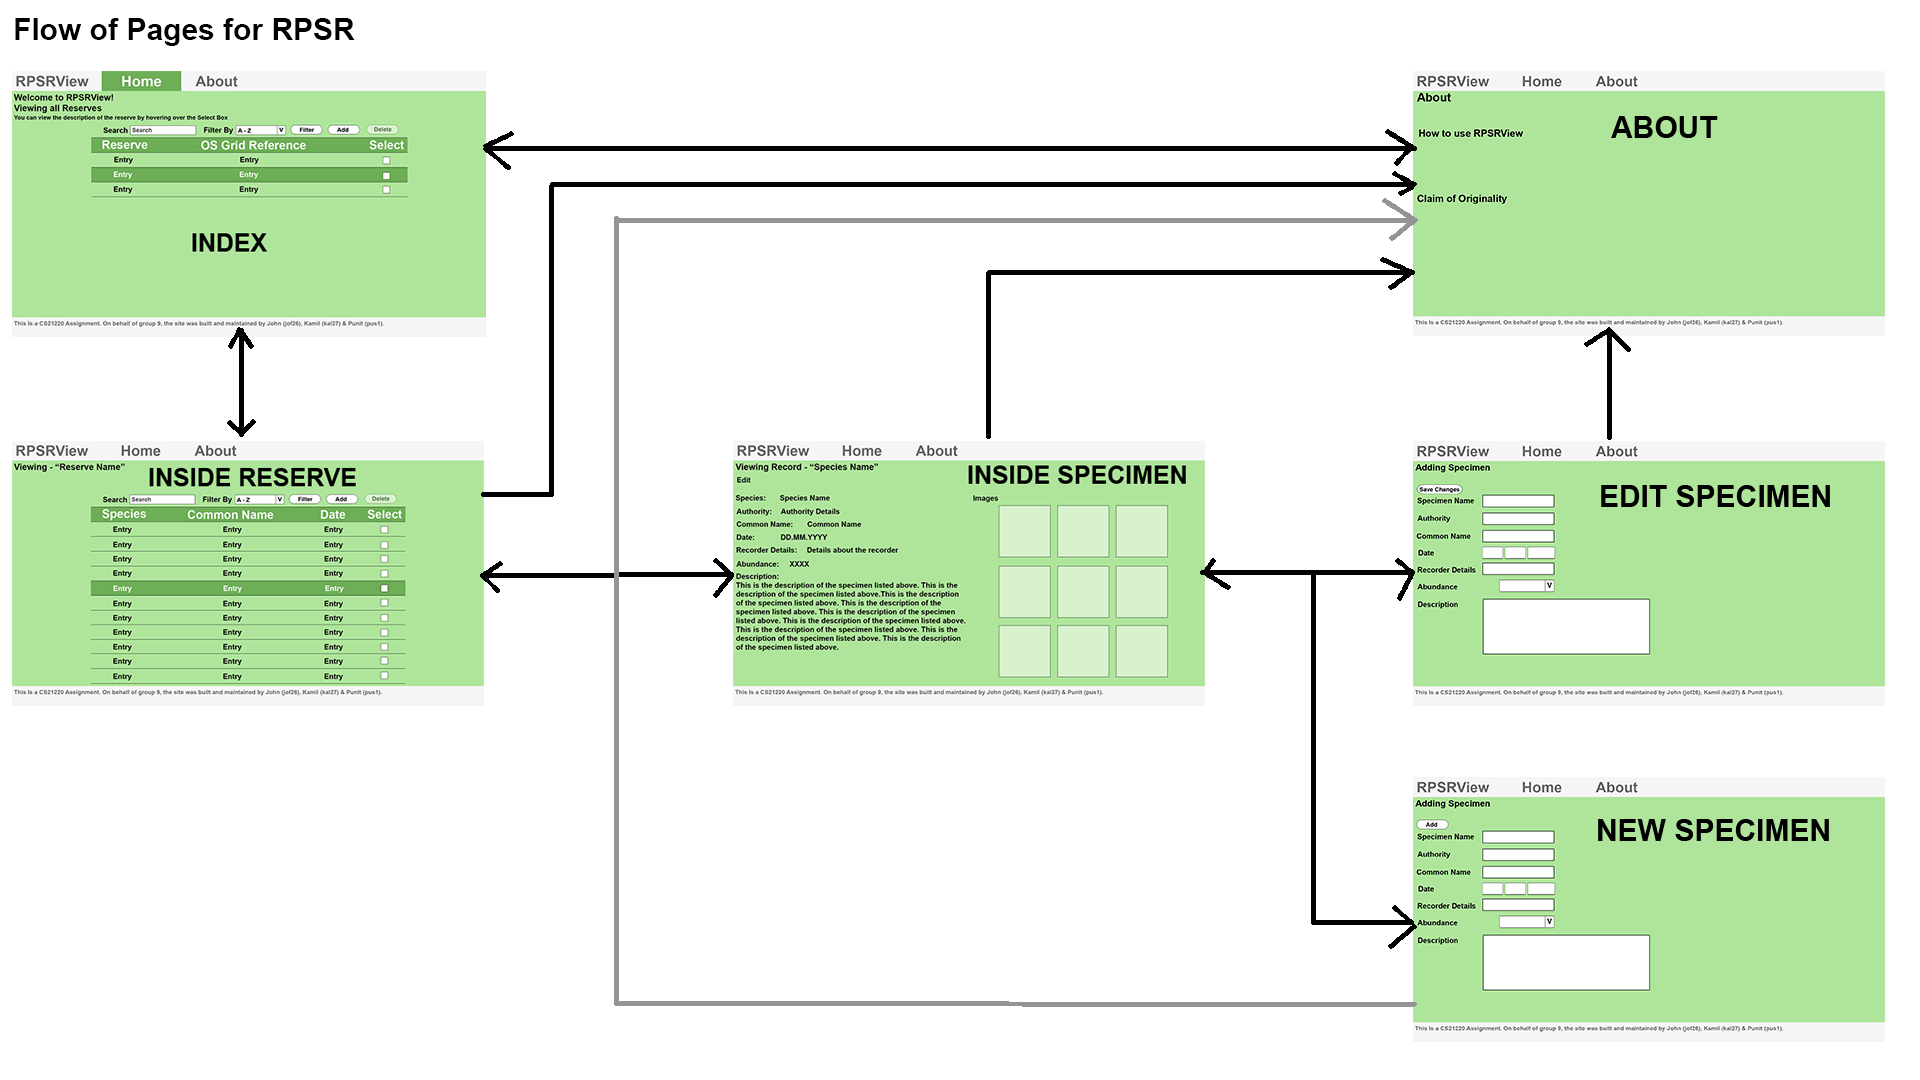
\includegraphics[scale=0.20]{web-FlowPLAN}
			\end{center}
			\caption{Page flow}
			\label{fig:pflow-page}
		\end{figure}

	\subsection{Android App Design}

		\begin{figure}[H]
			\begin{center}
				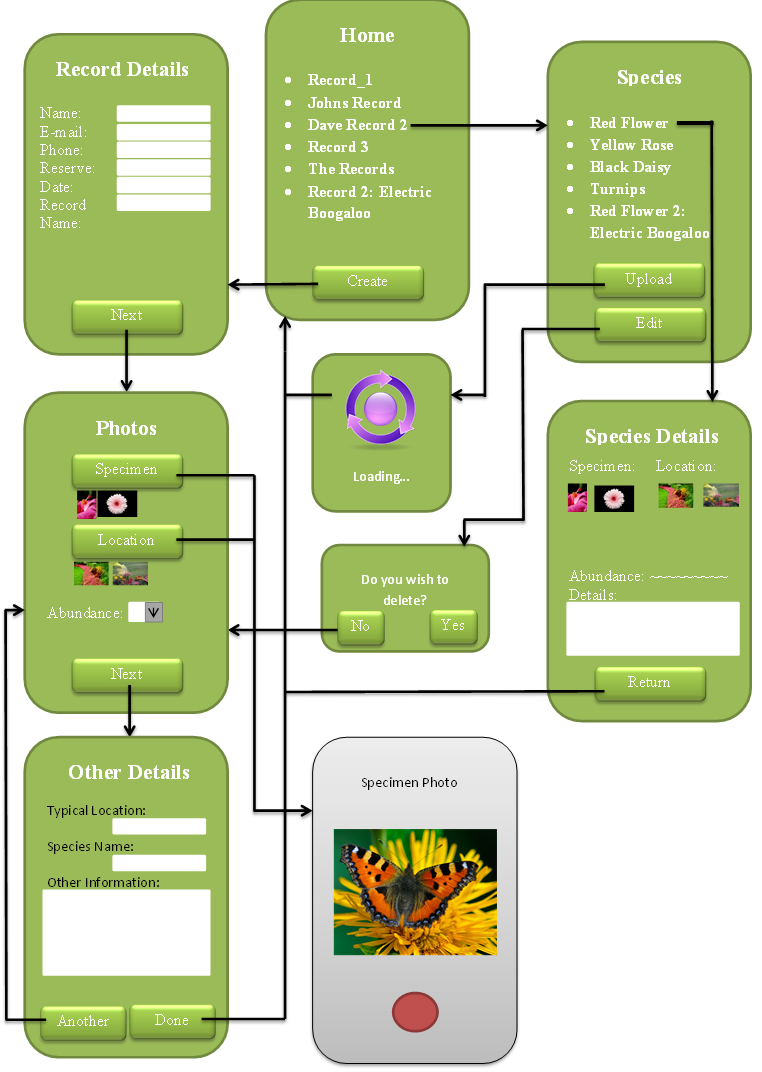
\includegraphics[scale=0.45]{app-PageFlow}
			\end{center}
			\caption{Page flow}
			\label{fig:app-pageflow}
		\end{figure}

		Figure~\ref{fig:app-pageflow} shows how each screen in the app is linked.

		The Home screen will contain a list of the current recordings that haven't yet been uploaded and a button to create a new one. 
		If the user presses the \textit{Create} button they will be asked to fill in the following forms to complete their recording:
		\begin{enumerate}
			\item They will first be asked to input their details and select a reserve - see Figure~\ref{fig:app-recdetails}.
			\item They will be asked to take a photo both for the specimen and the location it was found, as well as provide an abundance - see Figure~\ref{fig:app-photos}.
			\item They will then be asked to provide more details for the species - see Figure~\ref{fig:app-specdetailsentry}.
		\end{enumerate}
		Note: There is an option to input more than one species into the same recording, pressing the `Another' button will take you back to step 2.

		\begin{figure}[H]
			\begin{center}
				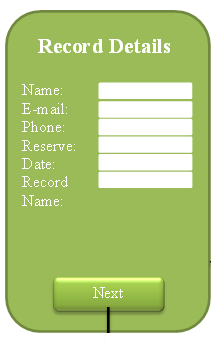
\includegraphics[scale=0.7]{app-RecorderDetails}
			\end{center}
			\caption{Entering recorder's details and reserve}
			\label{fig:app-recdetails}
		\end{figure}

		\begin{figure}[H]
			\begin{center}
				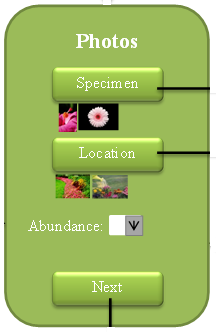
\includegraphics[scale=0.7]{app-Photos}
			\end{center}
			\caption{Providing photos and an abundance for a species}
			\label{fig:app-photos}
		\end{figure}

		\begin{figure}[H]
			\begin{center}
				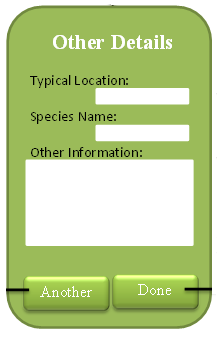
\includegraphics[scale=0.7]{app-OtherDetails}
			\end{center}
			\caption{Providing more details for a species}
			\label{fig:app-specdetailsentry}
		\end{figure}		

		Once completed the record can be saved to the device by pressing the \textit{Done} button, this will return the user to the \textit{Home} screen.

		\begin{figure}[H]
			\begin{center}
				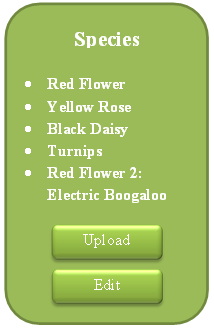
\includegraphics[scale=0.7]{app-SpeciesList}
			\end{center}
			\caption{List of recorded species saved to be edited or uploaded}
			\label{fig:app-specieslist}
		\end{figure}

		If the user selects one of the records in the list they will be taken to a screen (Figure~\ref{fig:app-specieslist}) which lists the species in the current recording and two buttons.
		These buttons are: \textit{Edit} and \textit{Upload}.
		\begin{itemize}
			\item Selecting the species will bring up the current details of that species including the pictures and abundance - see Figure~\ref{fig:app-speciesdetails}.
			\item Selecting `Upload' will send that record to the database. and then return the user to the Home screen.
			\item Upon selecting the `Edit' button, the user will be asked if they want to delete it. Selecting ``Yes'' takes them to the Home screen while ``No'' takes them to the beginning of the record creation (Figures~\ref{fig:app-recdetails}, \ref{fig:app-photos}, \ref{fig:app-specdetailsentry}) but this time all the fields are already filled in and editable.
		\end{itemize}

		\begin{figure}[H]
			\begin{center}
				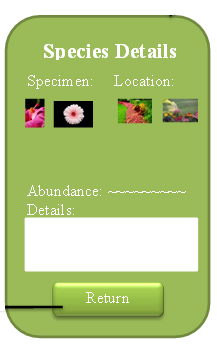
\includegraphics[scale=0.7]{app-SpeciesDetails}
			\end{center}
			\caption{The current details of a species selected from the list of recorded species}
			\label{fig:app-speciesdetails}
		\end{figure}

\section{Gantt Chart}
		\begin{landscape}
			\begin{ganttchart}[y unit title=0.4cm,
				y unit chart=0.5cm,
				vgrid,hgrid, the dfhs eu () 
				title label anchor/.style={below=-1.6ex},
				title left shift=.05,
				title right shift=-.05,
				title height=1,
				bar/.style={fill=green!100},
				incomplete/.style={fill=white},
				progress label text={},
				bar height=0.7,
				group right shift=0,
				group top shift=.6,
				group height=.3,
				group peaks height =.2
				]
				{1}{30}
				%labels
				\gantttitle{October}{12}
				\gantttitle{November}{12}
				\gantttitle{December}{6} \\ 
				\gantttitle{6th}{3} 
				\gantttitle{13th}{3}
				\gantttitle{20th}{3} 
				\gantttitle{27th}{3} 
				\gantttitle{3rd}{3} 
				\gantttitle{10th}{3} 
				\gantttitle{17th}{3} 
				\gantttitle{24th}{3}
				\gantttitle{1st}{3}
				\gantttitle{8th}{3}  \\
				%tasks
				\ganttbar{Project Plan}{1}{10} \\
				\ganttbar{Project Plan Delivery}{10}{10} \\
				\ganttbar{Test Specs}{10}{15} \\
				\ganttbar{Design specs}{16}{24} \\
				\ganttbar{0 - Role Delegation}{16}{18} \\
				\ganttbar{1 - GUI}{16}{24} \\
				\ganttbar{1.1 - App}{16}{24} \\
				\ganttbar{1.2 - Web}{16}{24} \\
				\ganttbar{2 - Database design}{16}{24}\\
				\ganttbar{3 - Backends}{16}{24}\\
				\ganttbar{3.1 - App}{16}{24}\\
				\ganttbar{3.2 - Web}{16}{24} \\
				\ganttbar{4 - Client + Server}{16}{24} \\
				\ganttbar{5 - Prototype Research}{16}{24} \\
				\ganttbar{6 - Prototype}{16}{24} \\
				\ganttbar{Deliver Prototype}{25}{25} \\
				\ganttbar{Dependancy Check}{25}{30} 

				%relations
				\ganttlink{elem0}{elem1} 
				\ganttlink{elem3}{elem4} 
				\ganttlink{elem4}{elem5} 
				\ganttlink{elem4}{elem6} 
				\ganttlink{elem4}{elem7}
				\ganttlink{elem4}{elem8} 
				\ganttlink{elem4}{elem9} 
				\ganttlink{elem4}{elem10} 
				\ganttlink{elem4}{elem11} 
				\ganttlink{elem4}{elem12}  
				\ganttlink{elem4}{elem13} 
				\ganttlink{elem4}{elem14}
				\ganttlink{elem5}{elem15} 
				\ganttlink{elem5}{elem16} 
				\ganttlink{elem6}{elem15}
				\ganttlink{elem6}{elem16} 
				\ganttlink{elem7}{elem15} 
				\ganttlink{elem7}{elem16} 
				\ganttlink{elem8}{elem15} 
				\ganttlink{elem8}{elem16}  
				\ganttlink{elem9}{elem15} 
				\ganttlink{elem9}{elem16} 
				\ganttlink{elem10}{elem15}
				\ganttlink{elem10}{elem16} 
				\ganttlink{elem11}{elem15} 
				\ganttlink{elem11}{elem16} 
				\ganttlink{elem12}{elem15} 
				\ganttlink{elem12}{elem16}  
				\ganttlink{elem13}{elem15} 
				\ganttlink{elem13}{elem16} 
				\ganttlink{elem14}{elem15} 
				\ganttlink{elem14}{elem16}  
			\end{ganttchart}
		\end{landscape}
		\newpage
		\begin{landscape}
			\begin{ganttchart}[y unit title=0.4cm,
				y unit chart=0.5cm,
				vgrid,hgrid, the dfhs eu () 
				title label anchor/.style={below=-1.6ex},
				title left shift=.05,
				title right shift=-.05,
				title height=1,
				bar/.style={fill=green!100},
				incomplete/.style={fill=white},
				progress label text={},
				bar height=0.7,
				group right shift=0,
				group top shift=.6,
				group height=.3,
				group peaks height =.2
				]
				{1}{21}
				%labels
				\gantttitle{January}{12}
				\gantttitle{February}{9}\\  
				\gantttitle{5th}{3} 
				\gantttitle{12th}{3} 
				\gantttitle{19th}{3} 
				\gantttitle{26th}{3} 
				\gantttitle{2nd}{3} 
				\gantttitle{9th}{3} 
				\gantttitle{16th}{3} \\
				%tasks
				\ganttbar{Implementation}{7}{9} \\
				\ganttbar{0 - Role Delagation}{7}{9} \\
				\ganttbar{1 - Android App}{7}{9}\\
				\ganttbar{1.1 - Local Storage}{7}{9}\\
				\ganttbar{1.2 - Database Links}{7}{9}\\
				\ganttbar{1.3 - HTTP proto}{7}{9} \\
				\ganttbar{2 - Website}{7}{9} \\
				\ganttbar{2.1 - Client side}{7}{9} \\
				\ganttbar{2.2 - Server side}{7}{9} \\
				\ganttbar{2.3 - Database Links}{7}{9} \\
				\ganttbar{3 - Unit Tests}{7}{9} \\
				\ganttbar{4 - Compliance Checks}{7}{9}\\
				\ganttbar{Testing}{7}{12}\\
				\ganttbar{1 - Stress Testing}{7}{12}\\
				\ganttbar{1.1 - Web Test App}{7}{12}\\
				\ganttbar{1.2 - App Test Web}{7}{12} \\
				\ganttbar{2 - Acceptance Testing}{7}{12} \\
				\ganttbar{3 - Bug Fixing}{7}{12} \\
				\ganttbar{Documentation}{13}{15}\\
				\ganttbar{1 - Product documentation}{13}{15}\\
				\ganttbar{2 - Project Report}{13}{15}
				%relations  
				\ganttlink{elem1}{elem2} 
				\ganttlink{elem1}{elem3} 
				\ganttlink{elem1}{elem4} 
				\ganttlink{elem1}{elem5} 
				\ganttlink{elem1}{elem6} 
				\ganttlink{elem1}{elem7} 
				\ganttlink{elem1}{elem8} 
				\ganttlink{elem1}{elem9} 
				\ganttlink{elem1}{elem10} 
				\ganttlink{elem1}{elem11}
				\ganttlink{elem2}{elem12} 
				\ganttlink{elem3}{elem12} 
				\ganttlink{elem4}{elem12} 
				\ganttlink{elem5}{elem12} 
				\ganttlink{elem6}{elem12} 
				\ganttlink{elem7}{elem12}  
				\ganttlink{elem8}{elem12} 
				\ganttlink{elem9}{elem12} 
				\ganttlink{elem17}{elem18} 
				\ganttlink{elem17}{elem19} 
				\ganttlink{elem18}{elem20} 
				\ganttlink{elem19}{elem20} 
			\end{ganttchart}
		\end{landscape}

\section{Risk Analysis}
	\subsection{Team Risks}
		\begin{center}
			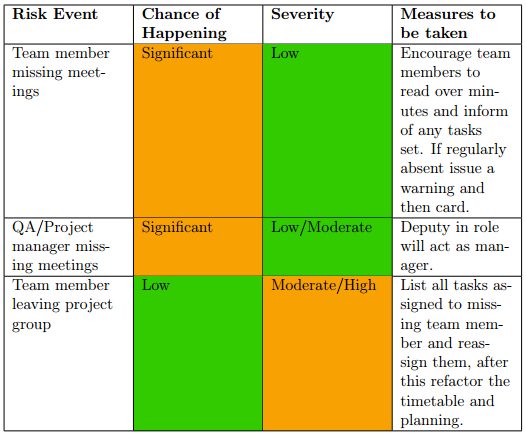
\includegraphics{Team_Risks}
		\end{center}

	\subsection{Project Risks}
		\begin{center}
			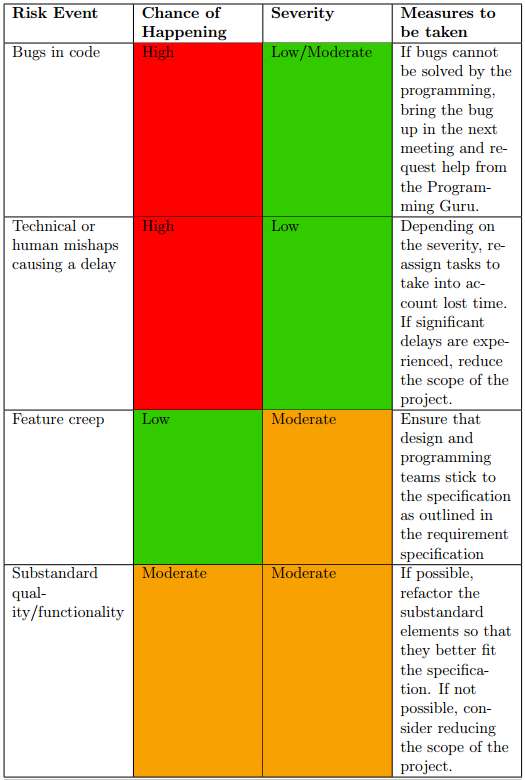
\includegraphics{Project_Risks}
		\end{center}

	\subsection{Client Risks}
		\begin{center}
			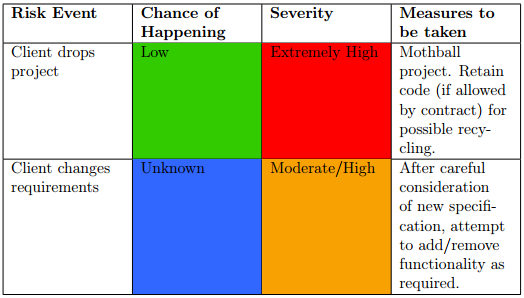
\includegraphics{Client_Risks}
		\end{center}

\section{References}
	N/A

\begin{versionhistory}
  \vhEntry{0.0}{21.10.14}{leh28}{Created document with structure and skeleton writeup}
  \vhEntry{1.0}{23.10.14}{leh28}{Updated with full-body text and screenshots}
  \vhEntry{1.1}{26.10.14}{leh28}{Minor updates after revisions decided upon in meeting}
  \vhEntry{1.2}{25.11.14}{jof26, leh28}{John rewrote website design, changes implemented by Leon}
  \vhEntry{1.3}{22.01.15}{pus1}{Updated use cases, added app screen designs to UI design section}
  \vhEntry{2.0}{25.01.15}{pus1}{Edited introduction, overview sections following feedback, added references section}
  \vhEntry{2.1}{09.02.15}{jac95}{Updated Gantt chart}
  \vhEntry{3.0}{12.02.15}{pus1}{Added header/footer and title page information in compliance with SE.QA.03}
\end{versionhistory}

\end{document}
